\chapter{Implementation}

\section{Cineast}

\subsection{Cineast core changes}
UV + texture support in meshes and OBJ loader

\subsection{Model Formats}

The current implementation supports the Wavefront OBJ [\todoMissing{Missing ref}] format as it is comparatively
simple to parse. However, the feature extraction algorithm is agnostic to the original 3D model format and only requires
a 3D mesh consisting of triangles and vertices that contain the following attributes: position and texture coordinates.
Because of Cineast's [\todoMissing{Missing ref}] modular nature it is possible to add parsers for other 3D model formats, or
to extend the currently existing parsers to also read the aforementioned vertex attributes, without having to alter
the feature extraction algorithm.

\subsection{ClusterD2+Color feature extraction}
%What, why (color support), explain assumptions made that were not covered by the paper


In order to compare two or more 3D models for similarity the algorithm must first identify or
extract information that is relevant for the calculation of the similarity metric.
A common way to do so is to reduce the 3D model into an N-dimensional real-valued feature vector which
contains only the most relevant information, or a reduced and compacted version thereof, for a similarity comparison. This feature vector can
then be used to compute a similarity metric, e.g. by calculating the L2 distance between feature vectors.

Since our application allows the user to color their sculptures it makes sense that similarity queries also
take color into account. Hence part of the color information must be contained in the feature vector.
The ClusterD2+Color algorithm described by [\todoMissing{Missing ref}], which was used in our application,
achieves this by creating random sample points on the 3D model's surface according to certain criteria and then
use those sample points to compute a feature vector.

\subsubsection{Sample generation}

Many isosurface polygonization algorithms, such as our non-adaptive CMS [\todoMissing{Introduce abbr before}]
implementation used in this application, can produce highly tessellated meshes. Opposite to that meshes exported by
3D modeling software are often optimized to have large triangles where the surface has little detail, and small triangles where
the surface is more detailed. Hence it is important that the sample point generation is mostly independent of the triangle sizes
of the mesh, so that meshes of varying levels of tessellation can be compared for similarity effectively.
The ClusterD2+Color algorithm achieves this by making the sampling directly proportional to the surface area of the triangles, hence a sample point
has a higher chance to be positioned on a large triangle, and a smaller chance to be positioned on a small triangle.
Before any sample points are generated the model is first scaled such that its total surface area equals 100.
After generating a certain number samples the result is a collection of samples that are uniformly distributed on the mesh's surface. The number of samples
is determined by a function of the integral of the absolute Gaussian curvature over the model's surface as described in [\todoMissing{Missing ref}].

\subsubsection{Sample Selection}

\begin{figure}
\centering
\captionsetup{width=0.8\textwidth}
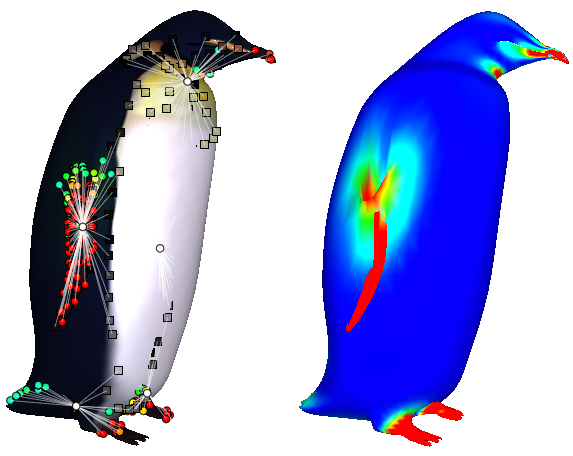
\includegraphics[width=0.5\textwidth]{feature_penguin.png}
\caption{Visualization of the sample selection and clustering. On the left is shown the textured input model and the resulting shape (circles) and color (squares) samples
and their cluster assignments (white circles and lines). The picture on the right shows the computed difference-of-Laplacian $D$ of the model (red: high, blue: low).}
\label{fig:feature_penguin}
\end{figure}

Once the initial samples have been generated they are filtered and tested for certain criteria.
These criteria differ between two different types of samples:

\subparagraph{Shape Samples}

\begin{wrapfigure}{R}{0.3\textwidth}
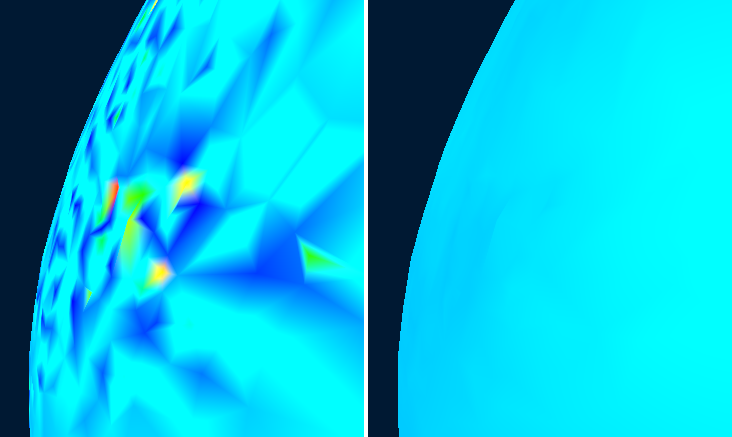
\includegraphics[width=0.3\textwidth]{laplacian_smoothing_artefacts.png}
\caption{$C^0$ (left) exhibits significant artefacts on a non-manifold mesh. $C^1$ (right) is a more sensible curvature map as baseline for the shown model.}
\label{fig:laplacian_smoothing_artefacts}
\end{wrapfigure}

These samples should convey relevant information about the geometric shape. Previous work done by [\todoMissing{Missing ref; Lee,C.H.,Varshney,A.,Jacobs,D.:Meshsaliency.In:ACMSIGGRAPH’05, pp. 659–666 (2005)}] has
shown that mean curvature is a good indication for visual saliency and thus for comparing geometric shapes for similarity. The mean curvature of the mesh vertices is computed using Taubin's method [\todoMissing{Missing ref}].
Our implementation of the ClusterD2+Color algorithm computes the mean curvature of each vertex and stores it as a vertex attribute. This mean curvature attribute is then smoothed over the mesh's surface
by a Laplacian smoothing approximation described by [\todoMissing{Missing ref; Implicit Fairing of Irregular Meshes using Diffusion and Curvature Flow}], resulting in a curvature map.
In particular, our implementation sets $\lambda = 8$ and, to satisfy the stability criterion $\lambda dt \leq 1$, $dt = \frac{1}{8}$, i.e. equivalently it applies small smoothings with $\lambda = 1$, $dt = 1$ a total of eight times for one
full smoothing operation. This is repeated multiple times to create three smoothed curvature maps $C^1$ through $C^3$. Each curvature map $C^i$ has been smoothed $i$ times. As opposed to [\todoMissing{Missing ref}] we use
$C^1$ as the baseline curvature map instead of $C^0$, because certain non-manifold (e.g. vertices or edges touching without being connected) models exhibit significant artefacts in $C^0$ as shown in Fig. \ref{fig:laplacian_smoothing_artefacts}. Lastly each shape sample calculates its $D = D^2 \oplus D^3$ value, where $D^i = C^i - C^{i-1}$ is the difference-of-Laplacian space, as shown in Fig. \ref{fig:feature_penguin}, and only the samples with the top 10\% highest $D$ values are kept. Indeed the remaining top
10\% $D$ value shape samples in Fig. \ref{fig:feature_penguin} are concentrated to the relevant features of the penguin model, namely its arms, feet and beak.

\subparagraph{Color Samples}

The color samples' purpose is to allow the algorithm to distinguish between models that have the same geometric shape but differ in
color or texture. This is achieved by only selecting those samples that lie on significant color transitions. As described by
Y.-J. Liu et al. [\todoMissing{Missing ref}], all generated samples extract the mesh's color at their position and then transform
the color to the CIE-LAB color space [\todoMissing{Missing ref}]. The resulting three CIE-LAB coordinates, $L*$, $a*$ and $b*$ are then
quantized into 6 ($L*$), respectively 4 ($a*$) and 4 ($b*$) integer values. These three, now quantized, coordinates are combined into a single color code integer, such that each of those color codes corresponds to a unique combination of the quantized coordinates. Similar colors are thus mapped to the same color code.\\
Lastly the algorithm only selects those samples as color samples of which less than $80\%$ of the neighboring samples' color codes are the same. In our implementation the neighborhood range is defined as a function of the model's mean edge length, or if less than 5 samples are found within said range then it chooses the 5 nearest samples as the neighborhood. In Fig. \ref{fig:feature_penguin} the
color samples are selected mostly along the transition between the white, black and beige hair of the penguin

\subsection{Comparing features for similarity}
%L2 norm, Jensen-Shannon divergence, $\chi^2$ distance

The selected shape and color samples now need to be reduced into an N-dimensional feature vector. ClusterD2+Color algorithm achieves this by first clustering nearby samples together and then
creating a histogram from the euclidean distances, i.e. L2 norm, between all samples that are not in the same cluster.\\

\begin{wrapfigure}{R}{0.3\textwidth}
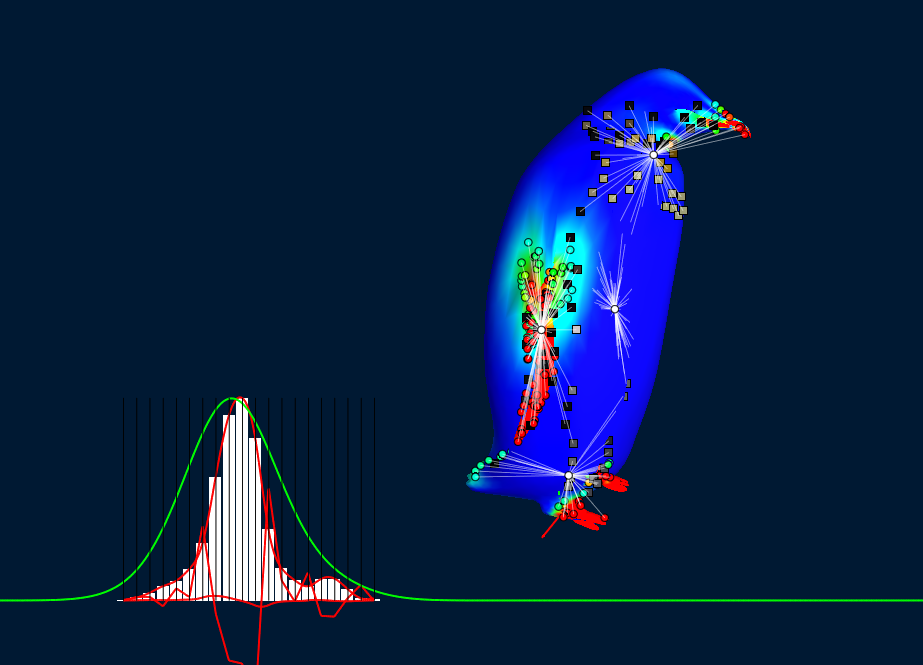
\includegraphics[width=0.3\textwidth]{feature_penguin_histogram.png}
\caption{The feature visualization tool that was developed during the feature extraction implementation. White: histogram feature vector. Green: probability density function of the histogram.}
\label{fig:feature_penguin_histogram}
\end{wrapfigure}

More specifically, the samples are clustered together using a modified
ISODATA algorithm described in [\todoMissing{Missing ref}]. In our implementation we set $P_n = 5\%$ \textit{of the total number of sample points}, $P_s = 2 * E$, $P_c = 10 * E$, $I = 100$ with $E =$ \textit{mean edge length of the model}.
Additionally we introduce two new parameters: $I_{min} = 10$, the minimum number of iterations, and $I_{nc} = 200$, the total maximum number of iterations after which the algorithm is stopped if no convergence is happening. Without
the $I_{min}$ parameter we have observed that the algorithm would commonly stop too early with inadequate cluster assignments. Then, once the samples are clustered together, the euclidian distances between all samples in different clusters
are computed and stored in an array. The values in this array are then normalized s.t. the lowest value in the array is mapped to zero and the highest value is mapped to one. Finally this array is then converted into a histogram with $20$
bins.\\
Y.-J. Liu et al. [\todoMissing{Missing ref}] have also proposed a second method called ClusterAngle+Color which calculates the values for the histogram from the angle between triplets of samples that are each in different clusters. According
to the authors this method results in a better similarity measure, however due to the $O(N^3)$ complexity we have unfortunately found it to be infeasible with the large number of samples generated from the user sculpted models in our application.\\
In either case the result is a histogram which serves as 20-dimensional feature vector and in fact, since they are a geometric signature of the model, they can be used to compare models for similarity,
e.g. by using the $\chi^2$ distance metric, a commonly used distance metric to compare two histograms for similarity. The lower the $\chi^2$ distance the more similar the models. Conveniently Cineast and its multimedia retrieval
database Cottontail DB\footnote{\url{https://github.com/vitrivr/cottontaildb}} offer an efficient k-nearest neighbors query for the $\chi^2$ distance metric.\\
Along with the $\chi^2$ distance metric the Jensen-Shannon divergence ($D_{JS}$), described by Y.-J. Liu et al. [\todoMissing{Missing ref}], was also implemented. In short, the $D_{JS}$ metric treats the histogram feature vector as an independent and identically-distributed sample of a random variable and thus first converts the histogram into a probability density function by using kernel density approximation with a gaussian kernel. The Jensen-Shannon divergence of the two probability density functions to compare is then computed and serves as a probabilistic measure ranging from 0 to 1 for how similar they are, so in a sense how likely it is that the two histograms were generated from the same model. Fig. \ref{fig:feature_penguin_histogram} shows the histogram of a penguin model and its probability density function, along with some debug information of curves required for the $D_{JS}$ calculation.


\subsection{REST API}

In order for a program to interface with Cineast's query capabilities an API is required. Cineast provides two main APIs, a WebSocket API and more importantly a REST API which was
used for the purposes of this thesis.\\
REST APIs, an acronym for Representational State Transfer, aim to communicate between to programs via requests and responses over the HTTP web protocol. The following, incomplete, list should give an insight
into how REST APIs operate - according to R. Fielding [\todoMissing{Missing ref; \url{https://www.ics.uci.edu/~fielding/pubs/dissertation/rest_arch_style.htm}}] REST APIs follow at least these following principles:
\begin{itemize}
	\item Client-Server: User interface concerns should be separated from data storage concerns.
	\item Stateless: Communication must be stateless. All information required for a request to be understood must be included in said request.
	\item Cache: Responses' data must be labeled whether the data can be cached on the client side or not. If it is chacheable the client may reuse the same data for future equivalent requests.
	\item Uniform Interface: The REST API should form a uniform interface. Said interface should remain the same independent of the back-end implementation.
	\item And several other principles.
\end{itemize}
Usually REST requests are exclusively executed by sending an HTTP GET, PUT, POST or DELETE request through certain server provided URLs. For example Cineast's similarity query endpoint has the following URL and is executed by
sending a POST request: \url{http://cineast.domain/find/segments/similar}. Additional data, such as the model to run the similarity query for, is included in the HTTP request body in the form of JSON data.\\
Throughout the course of development of this thesis Cineast's REST API was partially rewritten to use the Javalin\footnote{https://javalin.io/} web framework instead of Spark\footnote{http://sparkjava.com/} and SparkSwagger\footnote{https://github.com/manusant/spark-swagger}. Javalin makes great use of Cineast's already built-in JSON serialization structure using Jackson\footnote{https://github.com/FasterXML/jackson}. This enables Javalin, in combination with its OpenAPI plugin,
to generate an OpenAPI specification that describes Cineast's REST API in a standardized way. Moreover this OpenAPI specification allows programs like Swagger Codegen\footnote{https://swagger.io/tools/swagger-codegen/} to generate
fully functional code libraries in various programming languages capable of interfacing with the REST API defined by the specification. Since Javalin's OpenAPI plugin makes use of Jackson, it is capable of more reliably creating the specifications for JSON data structures than SparkSwagger, especially for subclasses of superclasses with generic types. The C\# library that was used to access Cineast's API endpoint from Unity was generated by the aforementioned OpenAPI
specification and Swagger Codegen.

\section{Voxels}

The foundation of the sculpting feature is based on voxels. In the most basic sense a voxel represents a value on a regular grid
in 3D space [\todoMissing{Missing ref; Wikipedia}]. These voxels are very useful to represent volumetric structures, such as sculptures
or terrain, since they fill the 3D space and each voxel represents one volume element.

\begin{wrapfigure}{R}{0.5\textwidth}
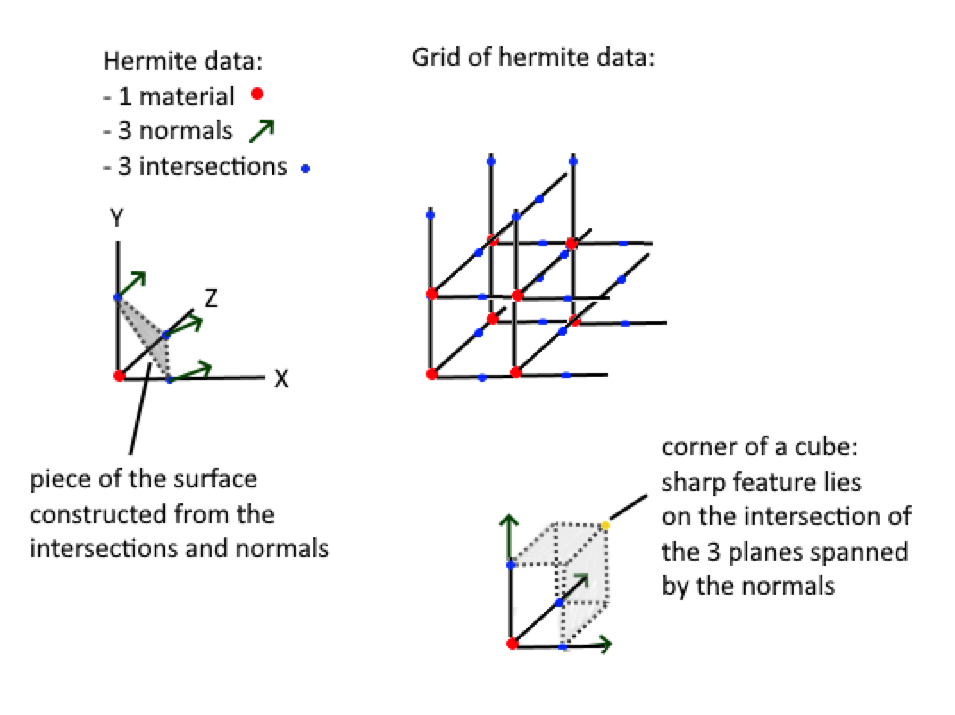
\includegraphics[width=0.5\textwidth]{hermite_data.png}
\caption{Hermite data.}
\label{fig:hermite_data}
\end{wrapfigure}

Since voxels are an abstract representation of volumes they can be visualized in various ways depending on the data the voxel contains.
Usually the data of a voxel consists of a single attribute, a color, in which case the voxel can be visualized e.g. by cubes, spheres, or splats.
More sophisticated voxels contain additional attributes such as normals or texture coordinates. In particular, our application uses voxels that
consist of a 32 bit material ID plus Hermite data [\todoMissing{Missing ref; Dual Contouring}]. Hermite data, first described by [\todoMissing{Missing ref; Dual Contouring}],
consists of two attributes: a material, exact intersection points and normals. Fig. \ref{fig:hermite_data} illustrates the Hermite data and how it can represent
diverse shapes. The Hermite data and voxel material provide enough information to construct the piece of surface represented by a voxel in the form of polygons.

\subsection{Voxel storage}

\todoMissing{Missing ref; Fig in Paper} %See below
\begin{wrapfigure}{R}{0.5\textwidth}
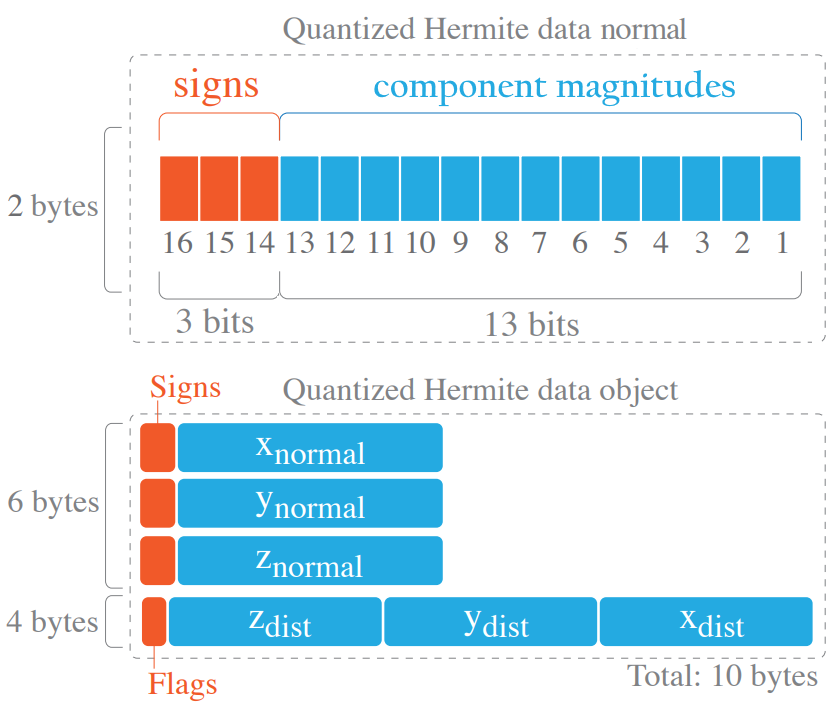
\includegraphics[width=0.4\textwidth]{quantized_hermite_data.png}
\caption{Quantized Hermite data structure. Top: a normal's component magnitudes are packed into 13 bits plus 3 bits for the signs. One normal thus fits into two bytes. Bottom: the entire quantized Hermite data object. $x,y,z_{dist}$ refer to the intersection points. Adapted from [XXX].}
\label{fig:quantized_hermite_data}
\end{wrapfigure}

There are many different data structures to store voxels, the simplest of which is simply storing the voxels' values in large 3D arrays.
Other data structures however need not necessarily store all voxel values on a regular grid. Often there are regions with many voxels of the same value, and
in that case it is beneficial to use a more advanced data structure that can store voxel values more memory efficiently.\\
The most common method to store voxels in memory is to split the voxels into fixed size blocks or chunks. Within each chunk the voxels are stored in an array. The chunks are stored seperately in a sparse data structure, e.g. a hash map,
where they can be accessed by their position. This gives a good trade-off between memory usage and access speed, because often voxel accesses happen within the same chunks and hence the hash map lookups can usually be cached. Instead of multi-dimensonal arrays for the chunk voxel storage we use one contiguous linear array per chunk to avoid having to dereference multiple pointers for a single access. The index into this linear array can be directly computed from a given X, Y and Z position within the chunk by the following formula: $index(x, y, z) = x * N * N + y * N + z$, where $N$ is the chunk size.
Our implementation uses a chunk size of $N=32$. Voxels on the faces towards the positive X, Y and Z axes are padding voxels that always mirror the state of the neighbour voxel in the respective neighbour chunk.
These padding voxels allow the voxel polygonizer to run faster since it entirely removes the need to query neighbour chunks during meshing. This method is described by [\todoMissing{Missing ref; A refined data addressing and processing scheme to accelerate volume raycasting}] in more detail. \\
As previously mentioned the voxels in this application consist of a 32 bit material ID plus Hermite data. Therefore the size of a single voxel in memory is: 4 (material) + $3*3*4$ (three normals, each with three 32 bit float components) + $3*4$ (three intersection points) = 52 bytes in total. Considering that a single chunk contains $32 * 32 * 32 = 32768$ voxels, hence consumes roughly 1.7MB, and one scene can contain many of these chunks,
the main memory will be exhausted rather quickly.
To remedy this issue the Hermite data compression scheme described by [\todoMissing{Missing ref; Fast and Adaptive Polygon Conversion By Means Of Sparse Volumes}] was used.
This quantized Hermite data compression is lossy since it relies on quantizing the floating point values into small integers that are then packed together using bitwise operations. The errors introduced by the compression are
negligible: the exact intersection points remain accurate to a $\frac{1}{1024}$th, respectively less than 0.1\%, of the voxel's edge length. Similarly the maximum error in a normalized normal's component is $\frac{1}{1024}$.
The effective size of the quantized Hermite data is 12 bytes (two of which are struct alignment padding), i.e. only 23\% of the uncompressed size. Fig. \ref{fig:quantized_hermite_data} shows the quantized Hermite data
structure in more detail.\\

\begin{wrapfigure}{R}{0.4\textwidth}
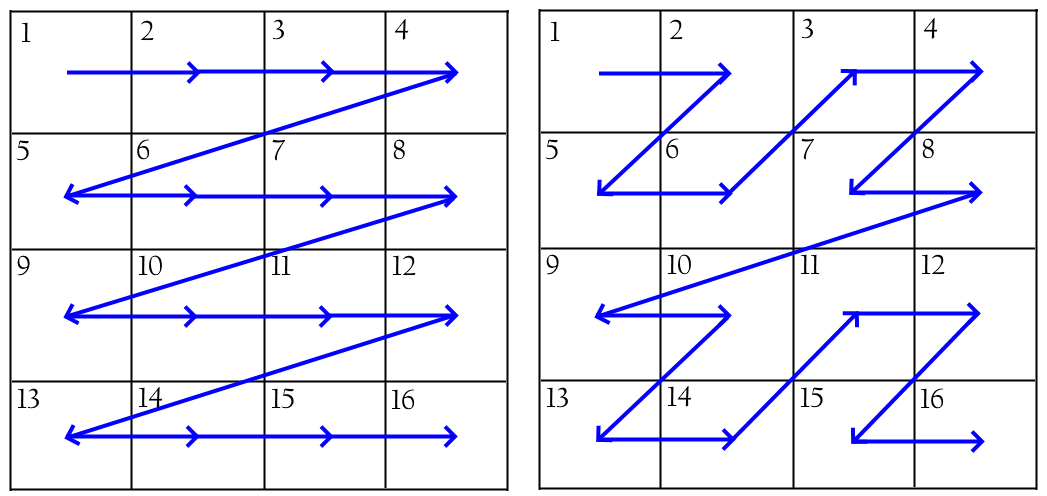
\includegraphics[width=0.4\textwidth]{indexing_order.png}
\caption{Simple linear indexing (left), Z-Order indexing (right). Each square represents a voxel in a 2D array. The blue line represents the order in which they are stored in main memory.}
\label{fig:indexing_order}
\end{wrapfigure}

A further potential optimization is to change the linear array indexing scheme. Modern CPUs have multiple cache layers - each cache layer is a fast memory unit and generally the faster the cache the less
memory it can store. When a program accesses a piece of memory from main memory the CPU loads the surrounding address space into a fixed size cache line, a contiguous piece of the heap memory around the access, into the cache.
If the program then accesses a nearby address again the CPU can read the value from the cache which is a lot faster than reading it from main memory. This is called a cache hit. On the other hand if the program accesses an address further away from the previous access than the size of a cache line the CPU will have to read the value from main memory instead, ergo a cache miss. Hence by optimizing for cache hits a program's speed can be improved if it is memory bound. The most
common access pattern for our voxel storage is to read eight neighbor voxels as a voxel cell for polygonization.
For simplicity's sake we will consider a 2D instead of 3D array: if we use simple linear indexing as shown in Fig. \ref{fig:indexing_order} to read the voxel cell (1, 2, 5, 6) there will be a large address difference between the voxels
on the first and second row. With large arrays this will often lead to cache misses. By instead using Z-Order indexing, also known as Morton indexing, spacially nearby voxels are much more likely to be nearby to each other in the address space, increasing the chance for cache hits. However, such indexing schemes usually have a larger overhead due to the calculation of the index. To compute the Z-Order indices parts of the Libmorton library\footnote{\url{https://github.com/Forceflow/libmorton}} were used and ported to C\#. Unfortunately in our case using Z-Order indexing has made no significant difference.\todoMissing{Validate this}


\subsection{CMS}

Since the voxels are just an internal volumetric representation some algorithm is required to convert them into something that a computer can
display on the monitor, e.g. a polygonal 3D mesh. From the group of iso-surface and surface polygonization algorithms we have decided to use the
Cubical Marching Squares algorithm described by [\todoMissing{Missing ref; CMS}].

\subsubsection{Multi-material extension for CMS}

\begin{wrapfigure}{R}{0.45\textwidth}
\begin{minipage}{0.45\textwidth}
\begin{algorithm}[H]
\caption{\textbf{GenerateSegment.} \textit{This procedure remains mostly the same as described in the CMS paper. The only difference is the last line \ref{algstatement:cms_generate_segment_change}.}}\label{alg:cms_generate_segment}
\begin{algorithmic}[1]
\Procedure{GenerateSegment}{Face $f$}
	\If{there are two segments}
		\State $\{l_1, l_2\} \gets $\Call{ResolveFaceAmbiguity}{$f$}
		\State $f.list \gets \{l_1, l_2\}$
		\State \Call{DetectFaceSharpFeature}{$f.list$}
	\ElsIf{there is one segment l}
		\State $f.list \gets \{l\}$
		\State \Call{DetectFaceSharpFeature}{$f.list$}
	\EndIf
	\State \Call{DetectMaterialTransition}{$f$} \label{algstatement:cms_generate_segment_change}
\EndProcedure
\end{algorithmic}
\end{algorithm}
\end{minipage}
\end{wrapfigure}

The regular CMS algorithm does not support multiple materials. Hence due to the need for multi material volumes in this thesis's application
a multi-material CMS extension was developed. In order for this to work the Hermite data normals must additionally also be stored for each material change edge, and not only for non-solid
to solid changes or vice versa. Furthermore each segment vertex must store a material.
Only one change was required in the algorithms shown in the CMS paper: \textsc{GenerateSegment}'s modification is shown in Alg. \ref{alg:cms_generate_segment}.
Since our application only uses regular voxel grids the modification was made to work on regular voxel grid cells. It can however be extended to work with the adaptive CMS version
in a similar manner.

\begin{algorithm}[H]
\caption{\textbf{DetectMaterialTransition.} \textit{This procedure finds and inserts material transitions into the segments of a face f. \textsc{InsertTransition} inserts the transition points into $f.list$ at their appropriate indices s.t. the segment's pieces remain straight and don't form folds, i.e. s.t. they subdivide the segment, and $transition2$ is to be inserted after $transition1$. The MATERIAL\_TRANSITION table returns the edge
connecting the two face corners with solid materials given the marching squares case.}}\label{alg:cms_detect_material_transition}
\begin{algorithmic}[1]
\Procedure{DetectMaterialTransition}{Face $f$}
	\If{$f.marchingSquaresCase$ is 2}
		\State $edge \gets $ MATERIAL\_TRANSITION[$f.marchingSquaresCase$]
		\State $normal \gets $\Call{GetNormal}{$f, edge$}
		\If{$normal \neq \varnothing$} \Comment{There can only be a transition if a normal exists.}
			\State $intersection \gets $\Call{GetIntersection}{$f, edge$}
			\State $tangent \gets $\Call{ConstructTangent}{$intersection, normal$}
			\ForAll{$l \in f.list$}
				\ForAll{$p \in l$} \Comment{The variable $p$ is one piece of the segment $l$.}
					\If{$tangent$ intersects with $p$}
						\State $transitionPoint \gets $\Call{IntersectionPoint}{$tangent, p$}
						\State $transition1 \gets $\Call{CreateTransition}{\null}
						\State $transition1.position \gets transitionPoint$
						\State $transition1.material \gets edge.points[0].material$
						\State $transition1.normal \gets normal$
						\State $transition2 \gets $\Call{CreateTransition}{\null}
						\State $transition2.position \gets transitionPoint$
						\State $transition2.material \gets edge.points[1].material$
						\State $transition2.normal \gets normal$
						\State \Call{InsertTransition}{$f.list, transition1, transition2$}
					\EndIf
				\EndFor
			\EndFor
		\EndIf
	\EndIf
\EndProcedure
\end{algorithmic}
\end{algorithm}


\begin{wrapfigure}{R}{0.5\textwidth}
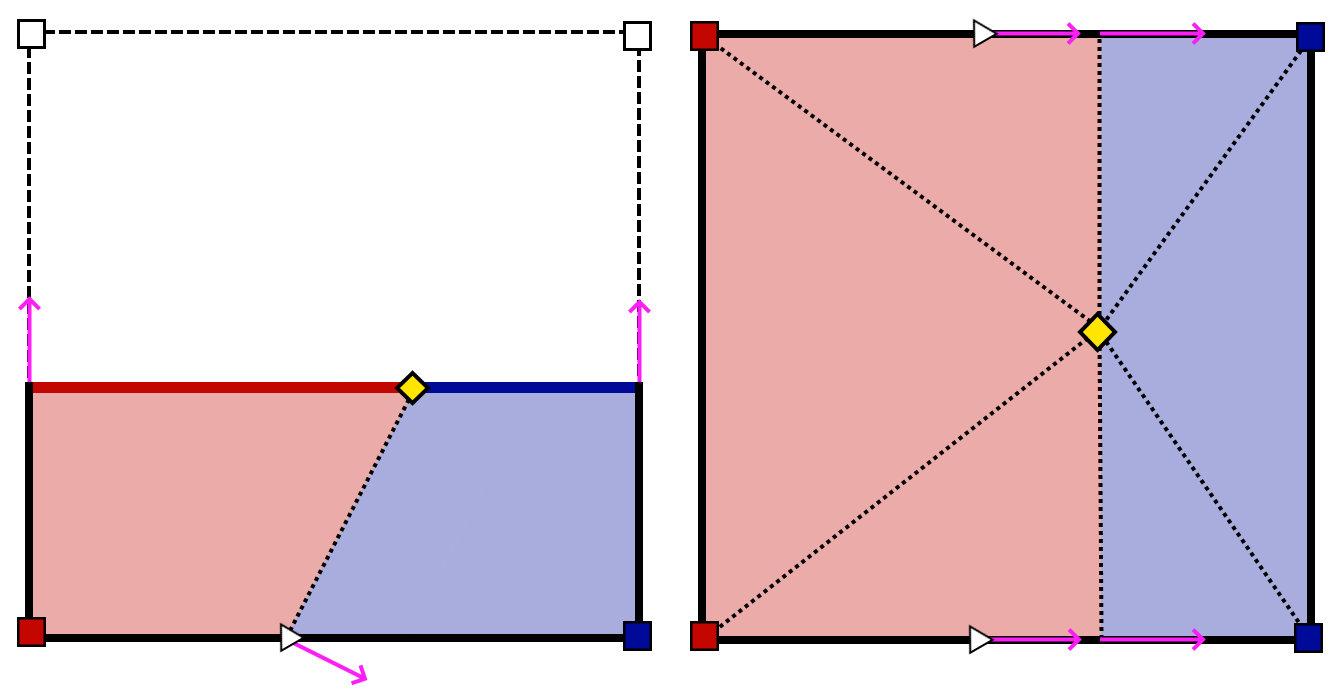
\includegraphics[width=0.5\textwidth]{cms_multi_material_side_top.png}
\caption{Multi-material CMS. The side view (left) shows how the material transitions (white triangles) are projected onto the segment, causing a split where one would expect the material transition to occur on the surface. The top view (right) shows how those splits are included in the sharp feature (yellow diamond) solution. The right side also shows the resulting triangulation (dotted lines).}
\label{fig:cms_multi_material}
\end{wrapfigure}

Additionally to the \textsc{GenerateSegment} modification the \textsc{DetectSharpFeature} implementation also requires a change. The transitions generated in \textsc{DetectMaterialTransition}, which are added to
$f.list$, and their normals must be included in the linear system of equations to be solved ([\todoMissing{CMS and Kobbelt et al.}]) for the sharp feature detection,
as suggested in [\todoMissing{Missing ref; DC paper}]. This causes the sharp feature to be placed where one would expect the material transition to occur on the surface, as shown in Fig. \ref{fig:cms_multi_material}.
This of course means that the multi-material CMS algorithm must always generate a sharp feature when material transitions are present, even if the sharp feature conditions/heuristics described by [\todoMissing{Kobbelt et al.}] are not met.

\subsubsection{Lookup table based implementation}

Much of the CMS algorithm can be done and perhaps be sped up using appropriate lookup tables, especially in the case of regular grid voxel cells. Indeed we have generated such lookup tables in order to show
the viability of a lookup table based approach. Due to time constraints and it breaking the previously mentioned multi-material extension however, it has ended up not being used in the final implementation.
Nevertheless with some more work it can also be made to work with multi-material volumes. Furthermore this lookup table based approach may prove useful for a future GPU based implementation as it splits
the problem into several small steps that can all be run in parallel with very little divergent behaviour.\\
A tool was implemented to generate the lookup tables for all $2^8 = 256$ possible cell states (two states per cell corner, solid vs. non-solid). Using rotational symmetries several lookup tables have been reduced in size - the initial lookup table maps one of the $256$ cell states to one of $23$ base configurations by rotating it appropriately (one or multiple $90^{\circ}$ rotations around the X, Y and Z axes). Each of the in total $24$ unique rotations gets its own index.
All other lookup tables are based on these base configurations, their components (in the context of CMS) and the rotation index.
From all the possible components that CMS can generate in a regular grid voxel cell, the lookup table tool has identified a total of $86$ unique components for all base configurations. These components have
then been indexed and their size and edges were stored in a seperate lookup table.\\

\begin{algorithm}[H]
\caption{\textbf{DisambiguationBit.} \textit{Determines the disambiguation bit for the specified base case and ambiguity number.}}\label{alg:cms_lt_disambiguation_bit}
\begin{algorithmic}[1]
\Procedure{DisambiguationBit}{int $baseCase$, int $ambiguityNr$}
	\State $tableIndex \gets baseCase * 6 * 4 + ambiguityNr * 4$
	\State $edges \gets \{$CASE\_AND\_AMBIGUITY\_NR\_TO\_EDGES[$tableIndex + 0$],
	\Statex ..., CASE\_AND\_AMBIGUITY\_NR\_TO\_EDGES[$tableIndex + 3$]$\}$
	\State $segment1 \gets $\Call{ConstructSegment}{$edges[0], edges[1]$} \Comment{Constructs a segment from the intersections on $edge[0]$ and $edge[1]$}
	\State \Call{DetectFaceSharpFeature}{$segment1$}
	\State $segment2 \gets $\Call{ConstructSegment}{$edges[2], edges[3]$}
	\State \Call{DetectFaceSharpFeature}{$segment2$}
	\If{$segment1$ intersects with $segment2$}
		\State \textbf{return} $1$
	\Else
		\State \textbf{return} $0$
	\EndIf
\EndProcedure
\end{algorithmic}
\end{algorithm}

One complication of the lookup table based approach are the potential 2D cell face ambiguities. All tables thus require as index not only the base configuration and rotation index, but also a $6$ bit disambiguation
index (one bit per cell face, also called "ambiguityRes"). For a given base configuration case and an ambiguity number (i.e. the index of the ambiguity to check, ranging from 0 to 5) Alg. \ref{alg:cms_lt_disambiguation_bit} calculates a
disambiguation bit. These disambiguation bits are then bit packed into a single integer where the bit with $ambiguityNr = 0$ is the most right bit and then from right to left according to $ambiguityNr$, resulting
in the $6$ bit disambiguation index. Although less common, the potential 3D ambiguities as mentioned in the CMS paper are not being handled by lookup tables, those still need to be resolved dynamically.\\
With the base configuration, rotation index and now also the disambiguation index a list of components can be obtained from yet another lookup table. The proposed lookup table based CMS algorithm then creates the segments for each
component, finds their 2D and 3D sharp features similarly to the regular CMS algorithm, and finally triangulates them.\\
In total the proposed lookup table based CMS algorithm primarily requires the following lookup tables which have been generated by our lookup table tool:
\begin{itemize}

	\item RAW\_CASE\_TO\_CASE\_ROTATION\_AND\_AMBIGUITY\_COUNT[$caseIndex * 3 + value$]\\
	Returns either the base configuration case, rotation index or ambiguity count
	\begin{itemize}
		\item $caseIndex$: One of the 256 possible cell cases
		\item $value$: 0 for base configuration case, 1 for rotation index, 2 for ambiguity count
  \end{itemize}
	
	\item CASE\_AND\_AMBIGUITY\_NR\_TO\_FACE[$baseCase * 6 + ambiguityNr$]\\
	Returns the base configuration face index (i.e. after reducing the rotational symmetries) for the given $ambiguityNr$
	\begin{itemize}
		\item $baseCase$: One of the $23$ base configuration cases
		\item $ambiguityNr$: Index of the ambiguity, as discussed above
  \end{itemize}
	
	\item ROTATION\_TO\_RAW\_FACES[$rotationIndex * 6 + baseFaceIndex$]\\
	Returns the original face index (i.e. before reducing the rotation symmetries)
	\begin{itemize}
		\item $rotationIndex$: One of the $24$ unique rotations
		\item $baseFaceIndex$: Base configuration face index
  \end{itemize}
		
	\item CASE\_AND\_AMBIGUITY\_NR\_TO\_EDGES[$baseCase * 6 * 4 + ambiguityNr * 4 + entry$]\\
	Returns the base configuration edge index (see Alg. \ref{alg:cms_lt_disambiguation_bit})
	\begin{itemize}
		\item $baseCase$: One of the $23$ base configuration cases
		\item $ambiguityNr$: Index of the ambiguity, as discussed above
		\item $entry$: Which edge index to return, i.e. 0 - 3 (four edges per face)
  \end{itemize}
	
	\item ROTATION\_TO\_RAW\_SIGNED\_EDGES[$rotationIndex * 12 + baseEdgeIndex$] \& 0b01111\\
	Returns original edge index (i.e. before reducing the rotation symmetries)
	\begin{itemize}
		\item $rotationIndex$: One of the $24$ unique rotations
		\item $baseEdgeIndex$: Base configuration edge index
  \end{itemize}
	
	\item CASE\_AND\_AMBIGUITY\_RES\_TO\_SIZE\_AND\_COMPONENTS[$baseCase * 64 * 5 + ambiguityRes * 5 + componentNr$]\\
	Returns the base configuration component index
	\begin{itemize}
		\item $baseCase$: One of the $23$ base configuration cases
		\item $ambiguityRes$: Disambiguation index, as discussed above
		\item $componentNr$: Which component to return, i.e. 1 - 4 (at most 4 configurations per voxel cell). If 0, the number of components in
		the voxel cell is returned.
  \end{itemize}

	\item COMPONENT\_TO\_SIZE\_AND\_EDGES[$componentIndex * 13 + edgeNr$]\\
	Returns the base configuration edge index
	\begin{itemize}
		\item $componentIndex$: One of the $86$ unique base configuration components
		\item $edgeNr$: Which component to return, i.e. 1 - 12 (at most 12 edges per component). If 0, the number of edges in
		the component is returned.
  \end{itemize}
	
\end{itemize}

For further details about the proposed lookup table CMS algorithm please refer to our lookup table tool and sample implementation written in Java.\todoMissing{Clean up and link somewhere}


\subsection{CSG operations on a voxel grid}
%How union and difference operations work on hermite data, algorithm

\begin{figure}
\centering
\captionsetup{width=0.8\textwidth}
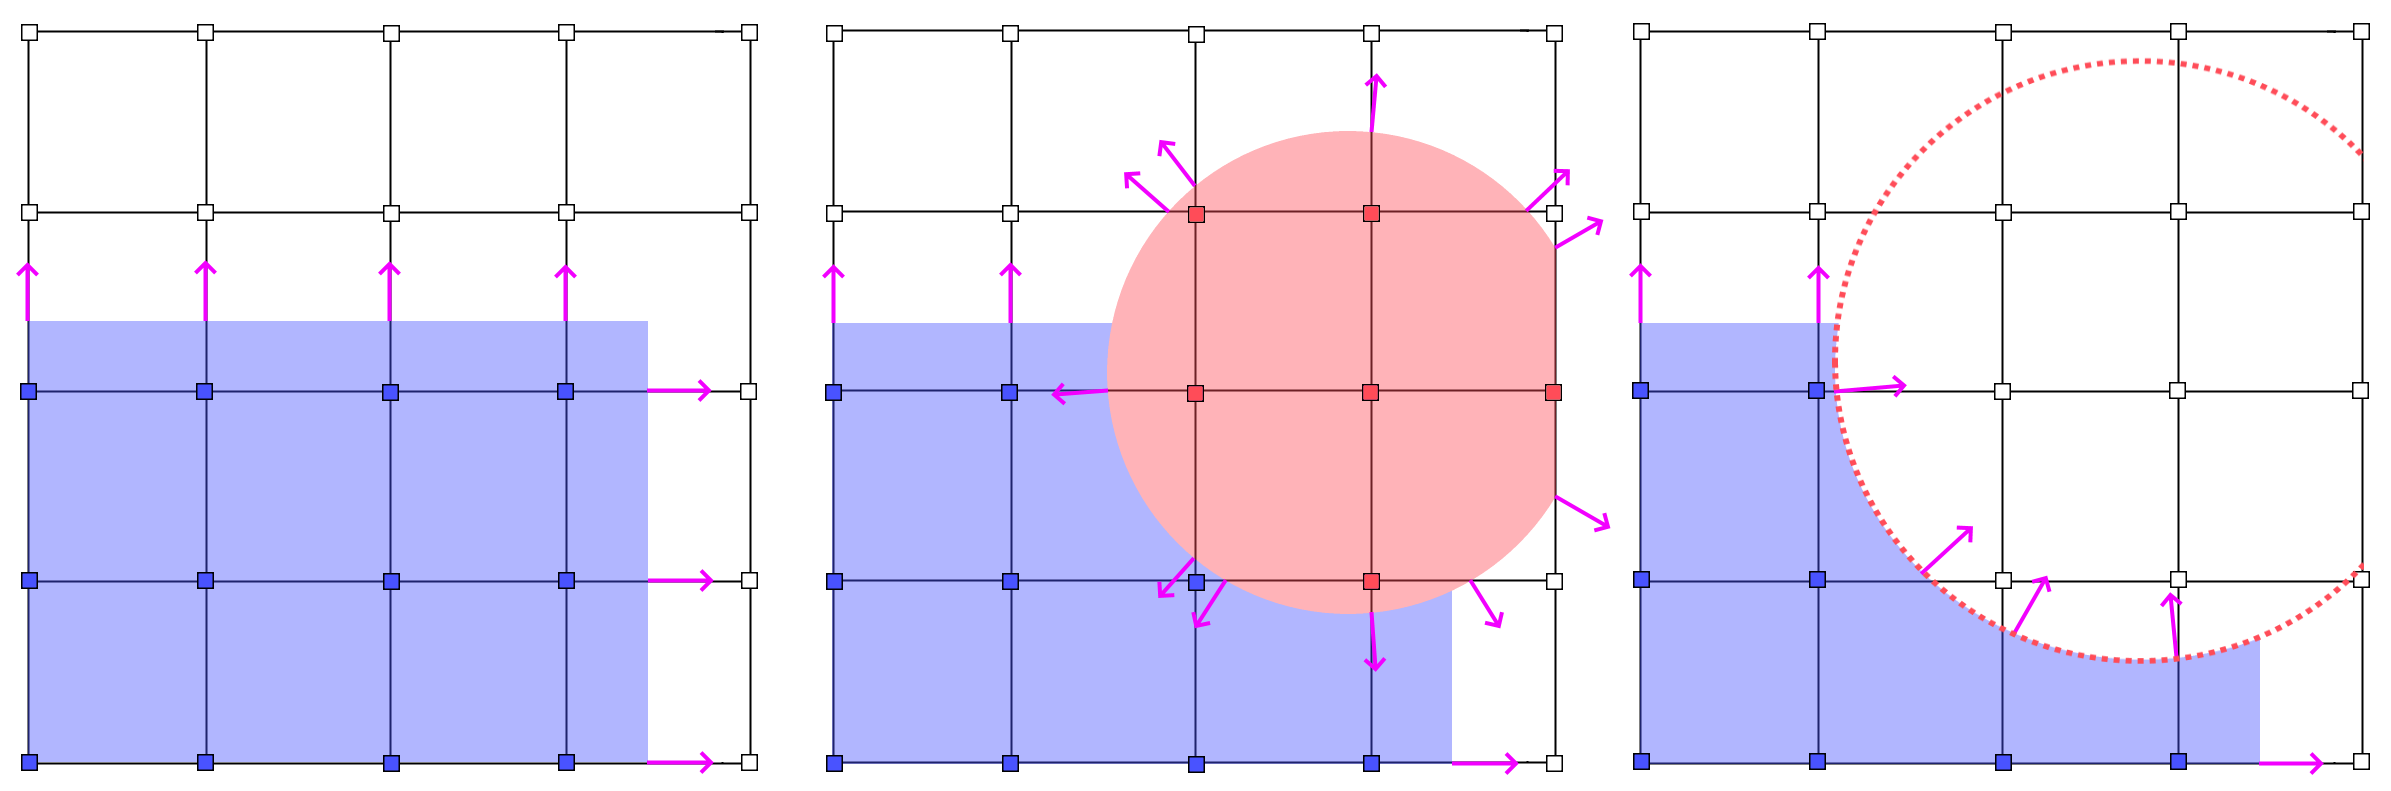
\includegraphics[width=0.8\textwidth]{hermite_data_csg.png}
\caption{CSG operations on a 2D Hermite data voxel grid. From left to right: initial grid, union and difference. Each square and its line segments to the right and above,
including any normals (pink) on them, represent one Hermite data voxel.}
\label{fig:hermite_data_csg}
\end{figure}

The CSG operations that our application uses for the sculpting brushes can be applied using variants of Alg. \ref{alg:hermite_data_csg}. 

\begin{algorithm}[H]
\caption{\textbf{Union.} \textit{Applies a CSG union to a voxel grid. \textsc{FindIntersection} finds the intersection of a primitive with the specified edge
and returns an intersection object. $intersection.distance$ is the distance between the intersection and a voxel or $edge.voxels[0]$, and $intersection.normal$ is the 
surface normal vector at the intersection.}}\label{alg:hermite_data_csg}
\begin{algorithmic}[1]
\Procedure{Union}{VoxelGrid $grid$, CSGPrimitive $primitive$}
	\ForAll{$v \in grid.voxels$}
			\If{$v$ is inside $primitive$}
				\State $v.insidePrimitive \gets true$
				\State $v.material \gets primitive.material$
			\Else
				\State $v.insidePrimitive \gets false$
			\EndIf
	\EndFor
	\ForAll{$e \in grid.edges$}
		\If{$e.voxels[0].insidePrimitive \neq e.voxels[1].insidePrimitive$}
			\State $intersection \gets$ \Call{FindIntersection}{$e, primitive$}
			\If{$e.voxels[0].insidePrimitive \cap intersection.distance \geq e.voxels[0].intersections[e.axis]$}
				\State $e.voxels[0].intersections[e.axis] \gets intersection.distance$
				\State $e.voxels[0].normals[e.axis] \gets intersection.normal$
			\ElsIf{$e.voxels[1].insidePrimitive \cap intersection.distance \leq e.voxels[0].intersections[e.axis]$}
				\State $e.voxels[0].intersections[e.axis] \gets intersection.distance$
				\State $e.voxels[0].normals[e.axis] \gets intersection.normal$
			\EndIf
		\EndIf
	\EndFor
\EndProcedure
\end{algorithmic}
\end{algorithm}

First the algorithm for a CSG union operation tags all voxels of the voxel grid whether they are inside the CSG primitive. Then it iterates over all edges of the voxel grid and checks if the two voxels
that form the edge have a different $insidePrimitive$ state. If that is the case then the edge must intersect with the primitive's surface and the exact intersection is found
using \textsc{FindIntersection}. Then the algorithm checks if any already existing intersections can and must be replaced by comparing their values. For multi-material voxel volumes some additional checks are required, mostly so that intersections are placed correctly at
solid to solid material transitions. In addition to that, our implementation also gives each CSG primitive an axis aligned bounding box, such that only those voxels and edges inside the bounding box need to be checked.\\
With some minor adjustments, namely swapping the $\geq$ and $\leq$, inverting the normals and changing the material assignment at the top to set to empty voxels, the algorithm for the CSG difference operation is obtained. \par

Previously it was mentioned that SDF's are well suited for CSG primitives.
The reason for this is that they are versatile and checking whether a voxel lies inside the SDF or finding
line to surface intersection points is simple. Checking whether a voxel is inside the SDF is a simple as checking whether the value of the SDF evaluated at said voxel is negative.
Finding intersection points (\textsc{FindIntersection}) on an edge is done by running a binary search on the edge, starting with the edge start- and endpoints and repeatedly moving them closer together.

\begin{wrapfigure}{R}{0.4\textwidth}
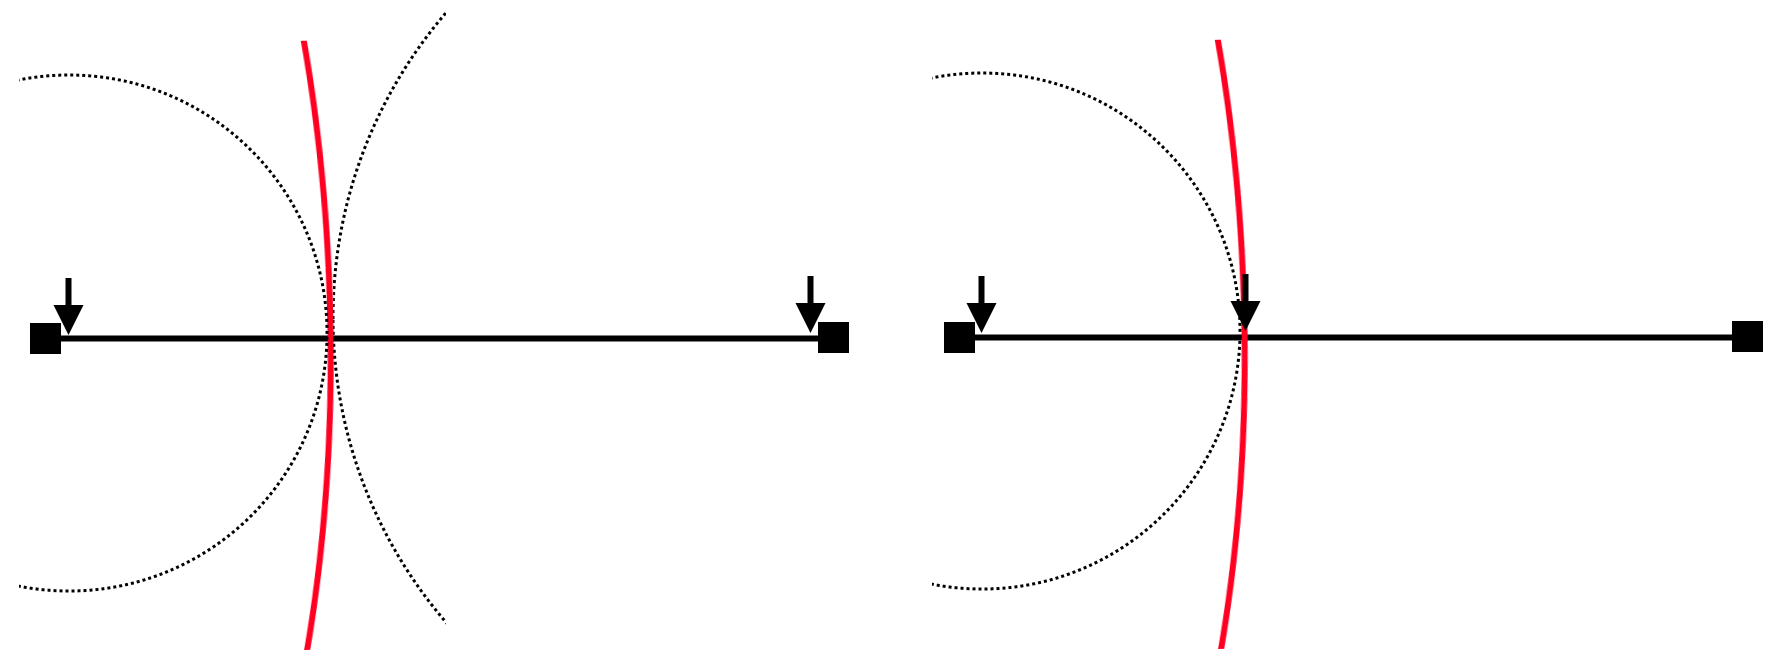
\includegraphics[width=0.4\textwidth]{adaptive_binary_search.png}
\caption{Adaptive binary search. Red circle: SDF's surface, Arrows: start- \& endpoint, Black circles: circles with radius of SDF's value at start- or endpoint. The adaptive binary search
finds the zero point from the initial state (left) after just one iteration (right).}
\label{fig:adaptive_binary_search}
\end{wrapfigure}

The binary search runs as long as the sign at the start- and endpoints are different, or until the value returned by the SDF for either start- or endpoint is within a certain threshold from zero. Both the start- and endpoints will thus converge towards the position where the SDF evaluates to zero, i.e. the SDF's surface.\\
This binary search can be optimized by using the values returned by the SDF for each iteration, since those values are a lower bound for the distance which the start- or endpoint can be moved along the edge without accidentally crossing the SDF's surface. Using this fact the adaptive binary search can make larger and more precise steps than a blind binary search. Consider a nearly linear surface perpendicular to the edge, like in Fig. \ref{fig:adaptive_binary_search}: the adaptive binary search will find the exact zero point after just one iteration because the two values returned by the SDF are the exact distances between the start- and endpoints and the surface. This may not always work for inexact SDF approximations since the returned values may not be actual lower bounds, hence the algorithm should still be able to use the regular binary search method as fallback for robustness.

\subsection{Rendering}
%Vertex colors encode material (RGB, A=texture id), texture array, triplanar texturing shader

\begin{wrapfigure}{R}{0.4\textwidth}
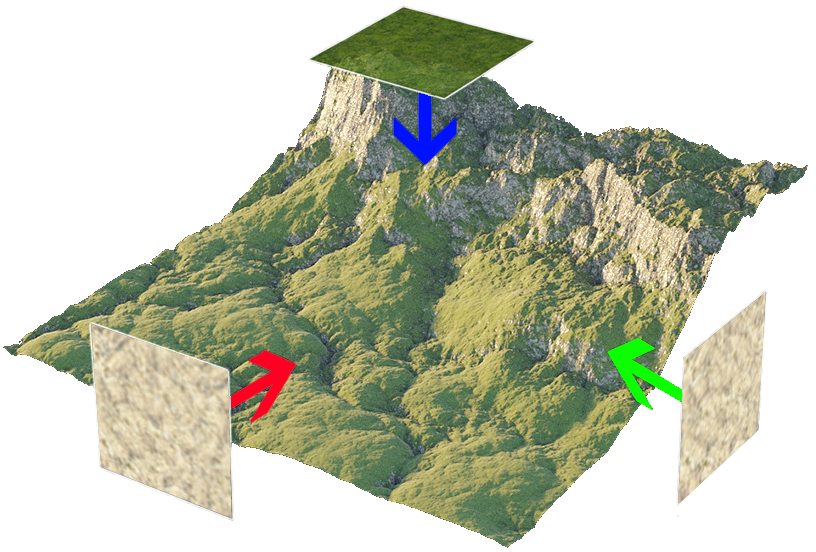
\includegraphics[width=0.4\textwidth]{triplanar_texture_mapping.png}
\caption{Tri-planar texture mapping of a mesh. Note how the hillsides of the terrain are rocky and the top is grassy.
Adapted from Corona Renderer\protect\footnotemark.}
\label{fig:triplanar_texture_mapping}
\end{wrapfigure}
\footnotetext{\url{https://corona-renderer.com/blog/wp-content/uploads/2017/04/Triplanar_01.jpg}}

The voxel polygonizer already does most of the heavy lifting for the voxel rendering. Once the voxel polygonizer has converted the voxels into a triangle mesh the rendering is done using the typical mesh rasterization techniques, provided by Unity, and shaders. The voxel materials and their colors are packed into the 32 bit RGBA color attachment of the mesh vertices. The first three components, RGB, are used to store the voxel color, the fourth component A for the voxel material ID.\\
Since our voxel meshes are not UV mapped, i.e. they do not contain information about where the textures should be sampled, we have resorted to a tri-planar texture mapping shader to texture them. These kinds of shaders use the position of a mesh's pixels to determine where to sample a texture, without the need of any explicit UV mapping. In order to achieve a realistic looking texture
mapping the tri-planar texture mapping shader projects an infinitely repeating texture from the X, Y and Z axes onto the mesh
like shown in Fig. \ref{fig:triplanar_texture_mapping}. The weight, i.e. how visible it is, of each texture projection is determined by the mesh's normals. For example the more a normal points along the X axis, the stronger the X axis texture projection is weighted, and the less the other two. The result of this is a mesh
that is usually textured nicely on all sides. In certain situations, especially when the weights of two texture projections are similar, e.g. for $45^{\circ}$ diagonal parts of the mesh with respect to axes, there can be unnatural overlapping of two texture projections. This however is only a problem for textures with obvious structures, e.g. bricks, as opposed to natural or noisy textures like e.g. dirt or grass.

\subsection{Voxelizer}
% Purpose, explain method used for voxelization (assigning triangles to bins, patching holes, etc.), use of job system

The precursor of our application already had an implementation of a voxelizer, however throughout the development of this thesis
the voxelizer was rewritten to scale better with high triangle counts.\\
The implementation of a basic voxelizer is described in Alg. \ref{alg:voxelize}. This algorithm however will only work properly
for meshes without holes.


\begin{algorithm}[H]
\caption{\textbf{Voxelize.} \textit{Voxelizes the given mesh into the voxel grid. \textsc{FillSection} fills the voxel grid along and inside the given section with the given material and also sets the voxel Hermite data at the section's start and end points.}}\label{alg:voxelize}
\begin{algorithmic}[1]
\Procedure{Voxelize}{VoxelGrid $grid$, Mesh $mesh$, Material $material$}
	\ForAll{$axis \in \{X,Y,Z\}$}
		\ForAll{$voxel \in grid.sideVoxels[axis]$}
			\ForAll{$section \in $ \Call{FindSections}{$axis, voxel.position ,mesh$}}
				\State \Call{$FillSection$}{$grid, section, material$} 
			\EndFor
		\EndFor
	\EndFor
\EndProcedure
\end{algorithmic}
\end{algorithm}

\begin{algorithm}[H]
\caption{\textbf{FindSections.} \textit{Finds all intersections of a line with the mesh and then returns all sections that are between an ingoing and outgoing intersection, i.e. inside the mesh.}}\label{alg:find_sections}
\begin{algorithmic}[1]
\Procedure{FindSections}{Axis $axis$, Position $position$, Mesh $mesh$}
	\State $line \gets$ \Call{CreateLine}{$position, position + axis * gridSize$}
	\State $intersections \gets \varnothing$
	\ForAll{$triangle \in mesh$}
		\State $intersections \gets intersections$ $\cup$ \Call{FindIntersection}{$line, triangle$}
	\EndFor
	\State \Call{Sort}{$intersections$}
	\State $sections \gets \varnothing$
	\State $previous \gets \varnothing$
	\State $inside \gets false$
	\ForAll{$intersection \in intersections$}
		\If{$\neg inside \cap previous \neq \varnothing$}
			\State $sections \gets sections$ $\cup$ \Call{CreateSection}{$previous,intersection$}
		\EndIf
		\State $previous \gets intersection$
		\State $inside \gets \neg inside$
	\EndFor
	\State \textbf{return} $sections$
\EndProcedure
\end{algorithmic}
\end{algorithm}

Essentially the algorithm checks the grid lines perpendicular to the +X, +Y and +Z faces of the voxel grid for intersections
with the mesh. Doing this for all the three grid faces will ensure that no triangles or voxels to be filled are missed.
The found intersections are then sorted from minimum distance from grid face to maximum distance. When iterating over these
sorted intersections the algorithm alternates between inside the mesh and outside the mesh, since for each incoming intersection
the next intersection must be an outgoing intersection. All voxels inside such a pair of ingoing and outgoing intersections are
then filled with a chosen material. For the first and last voxel in such a section the algorithm also needs to set the Hermite data (i.e. the voxel intersection values and normals).\\
We have found that in practice some triangles seem to be missed during the intersection checks due to floating point precision errors. To address this problem our implementation performs a post-processing
hole patching algorithm that checks for missing normals in the voxel Hermite data and then obtains them by sampling from the closest
triangle to the hole's position.\\
Note that the complexity of the algorithm, disregarding \textsc{FillSection}, is $O(N^2 * K)$ where $N$ is the voxel grid
size and $K$ the triangle count of the mesh, since for each side voxel (i.e. those touching one of the grid's +X, +Y or +Z faces, $3*N^2$ in total) the algorithm needs to check all triangles. For large $N$ and $K$ this poses a problem. Hence as improvement our new
algorithm first runs Alg. \ref{alg:assign_triangles}.

\begin{algorithm}[H]
\caption{\textbf{AssignTriangles.} \textit{Projects the AABB's of all triangles onto all three voxel grid faces and then
assigns the triangles to the bin of the according face and position.}}\label{alg:assign_triangles}
\begin{algorithmic}[1]
\Procedure{AssignTriangles}{Bins $bins$, Mesh $mesh$}
	\ForAll{$axis \in \{X,Y,Z\}$}
		\ForAll{$triangle \in mesh$}
			\State $box \gets$ \Call{CreateAABB}{$triangle$}
			\State $area \gets$ \Call{ProjectOnGridFace}{$axis,box$}
			\ForAll{$position \in area$}
				\State $bins[axis][position] = bins[axis][position] \cup triangle$
			\EndFor
		\EndFor
	\EndFor
\EndProcedure
\end{algorithmic}
\end{algorithm}

Following that Alg. \ref{alg:find_sections} is then modified to only iterate over the triangles in $bins[axis][position]$.
In practice this provides a good speed improvement, although at the cost of more memory, because Alg. \ref{alg:find_sections} will
only have to check a tiny fraction of all the triangles for each position.\\
In our implementation \textsc{FindSections} runs in parallel for all the voxels touching one grid face since all the voxels along one
of the face's perpendicular grid lines can be written to independently in parallel. This is done three times, once per grid face, because otherwise the algorithm could potentially write to the same voxel multiple times at the same time, causing a write conflict.

\section{VR Sculpting}

\subsection{Sculpting features}
General overview of capabilities and functionality, UIs, SteamVR Plugin, etc.

\subsection{Brush properties menu}
Functionalities, color selection (why HSV: you can see most colors at once, as opposed to RGB sliders)

\subsection{Custom brush editing menu}
Explain custom brush tool, why it exists, etc.